\documentclass[11pt]{article}
\usepackage[margin=1in]{geometry}
\usepackage{graphicx}
\usepackage{subcaption}
\usepackage{caption}

\title{GPU accelerated ray tracing}
\author{William Zhang}
\date{\today}

\begin{document}
\maketitle
\section{Design}
\subsection{Serial Implementation}
My serial raytracer implements support for secondary rays such as reflection and refraction and
shadow and distance attenuation of light intensity through objects. For each pixel, a ray is propagated
throughout the scene and checked for collisions with any objects. On collision, a \textit{shadow ray} is 
spawned towards every light source to calculate the degree in which the object is obscured from a nearby
light source. The \textit{secondary} reflection and refraction rays are spawned recursively should the collided object be 
transluscent or reflective. Contributions are all additive, but clamped to be in the range $[0.0, 1.0]$.
The final values are scaled to 255 to determine the value for each color channel. I support all 4 color
channels of the RGBA system, albeit the alpha channel is rarely set to a value different than 1.

Each object is represented as a collection of triangles that form a \textit{trimesh}. I chose triangles as the only
primitive to implement as every other primitive can be represented with triangles, including round objects such
as spheres through careful manipulation of triangle normal vectors. Each triangle component of an object is free
to have unique material properties, supporting complex object types. Objects can be duplicated with little cost by 
providing transformations such as translation and rotation to them. I also assume all objects have no gaps, and that
there are no objects within other objects.

In addition, I implement a bounding volume heirarchy (BVH) tree to prune a large portion of objects to perform collision
detection. A BVH tree is a binary tree that generates bounding boxes for nearby objects as a collective such that
if a ray misses the encompassing bounding box, it is guaranteed to miss all objects within it. Each leaf node of
the binary tree represents a specific scene object, while each inner node consists of a bounding box that encompasses
all its descendants. I constructed BVH trees by first sorting the objects by a space filling curve and then 
merging bottom-up between adjacent nodes.

\subsection{Parallel Implementation}
 My implementation consists of writing \textit{kernels} to be processed on the GPU. Kernel helper functions are annotated with \texttt{\_\_device\_\_} 
 and kernel entry functions are annotated with \texttt{\_\_global\_\_}. Functions need to be annotated on whether they reside on the host or the gpu 
 as GPUs use a different instruction set so compilation is different. Also, common library functions such as feeding into \texttt{std::cout} are not
 accessible on the GPU, so the different annotations enable the compiler to throw useful error messages. Launching kernels envokes each function in 
 parallel, where each instruction is loaded at the same time using different sets of registers. As such, using different values in the registers 
 allow for different colors to be computed per pixel despite using the same instruction stream.

My parallel raytracer implements the same features as the serial one. To support secondary rays, all recursion is
converted to an iterative counterpart, where state is stored on a stack and transitions between states are coded explicitly.
Likewise, BVH iteration was performed iteratively as well. Iteration must be used as although modern GPUs support recursion,
compilers cannot statically determine parameters such as the stack size. Stacks also reside in local memory, which
has high latency as it resides off chip.

In addition, my implementation uses the texture cache to store triangle vertices and normals. Although most GPUs have a designated
vertex cache, CUDA does not expose it. The texture cache is optimized for constant memory and the local coordinates of the triangle 
vertices never change irregardless of transformations, making it the next best choice. The texture cache does also support features
such as linear interpolation on the hardware, but in this project, I did not use those features.

Parallelization of raycasting simply involved broadcasting a ray per pixel as explained previously. BVH generation was parallelized
by using the Thrust library to sort by Morton code, then doing a reduction per level until the tree was constructed. In other words, adjacent nodes
were merged bottom up until $2n-1$ nodes were eventually constructed.

\section{Results}

\begin{figure}
    \begin{subfigure}[b]{0.3\textwidth}
    \centering
    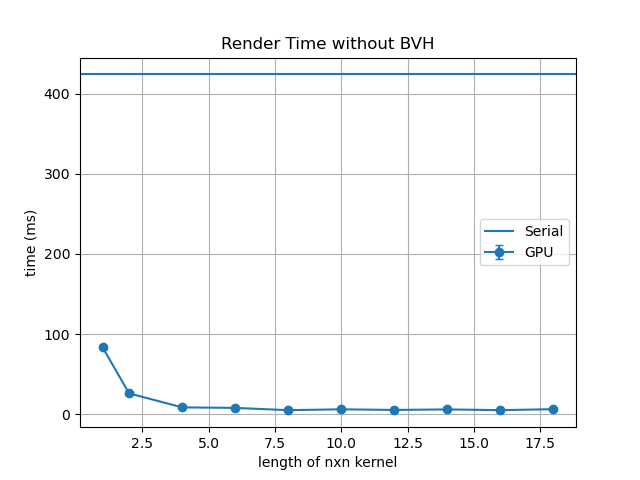
\includegraphics[scale=.3]{world1b1.png}
    \caption{Large speedups immediately apparent prior to BVH integration. Error bars indicate standard deviation.}
    \label{fig:no_bvh}
    \end{subfigure}
    \begin{subfigure}[b]{0.3\textwidth}
    \centering
    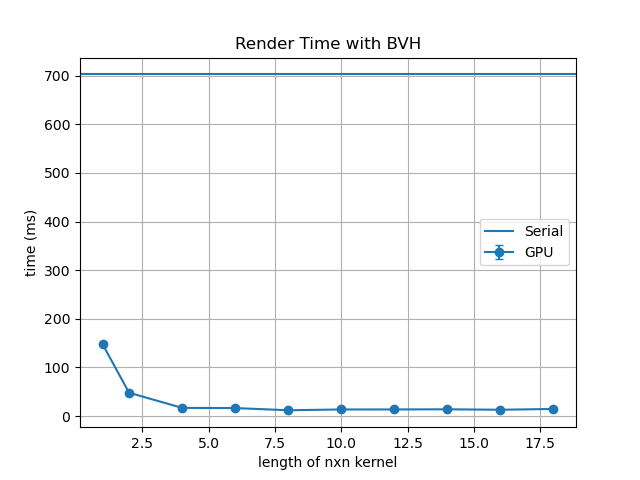
\includegraphics[scale=.3]{world8b8.png}
    \caption{Similar speedups with BVH integration.}
    \label{figure:bvh}
    \end{subfigure}
    \begin{subfigure}[b]{0.3\textwidth}
    \centering
    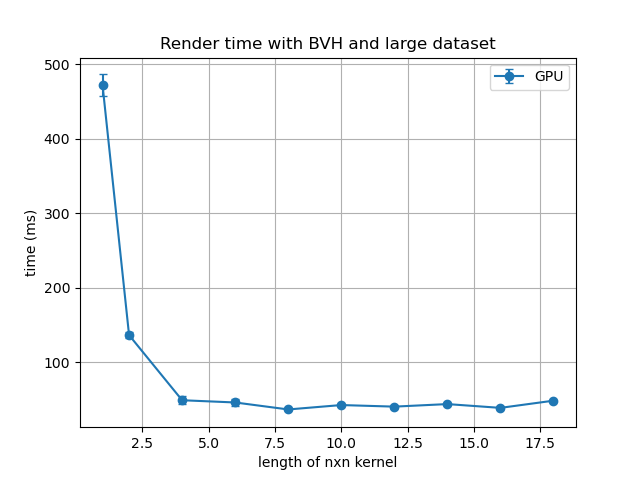
\includegraphics[scale=.3]{world16b16.png}
    \caption{Larger dataset with BVH integration.}
    \label{figure:large}
    \end{subfigure}
\end{figure}

GPU accelerating the process demonstrated remarkable speedup. As shown in Figure~\ref{fig:no_bvh}, even with a one by one block, a four-time speedup was
observed. This initially surprised me, but as the GPU can schedule each one by one block to a different streaming multiprocessor, parallelism can still be
achieved. I was also surprised by the result since I was initially under the impression that GPU cores were significantly slower than their CPU counterparts
to gain any speedup with a low number of threads. The asymptotic decrease does confirm to me of strong scaling confirming my first hypothesis. However, it does
not appear that the kernel dimension was very important, as increasing the block size at a certain part did not cost anything. BVH integration surprisingly closed 
the gap a little, but the same trends are seen (Figure~\ref{figure:bvh}).

\section{Limitations and Future Work}
Shared memory was not utilized at all during the implementation of this project. Due to the large size of metadata associated with collisions
and objects, at this time, I could not determine when it would be useful to use. To reach desired speeds, it is imperative that the ray tracer
eventually exploits it in the future. In addition, more complex features have not yet been implemented, such as caustics, constructive solid geometry,
and texture mapping.

\end{document}